\chapter{\textsc{Analyse du procédé de deux bacs d'eau avec régulation}}
\section{\textsc{Le procédé}}
	
	\paragraph{} Le système représenté sur la Figure 3 est composé de deux bacs cylindriques de section $S$. Ils sont reliés par un tuyau d’écoulement de section $S_n << S$. Le dernier bac se vide par un cylindre (également de section $S_n$ )
dans un réservoir situé sous les bacs. Une pompe de débit $Q(t) = K_debit u(t)$ permet de remplir respectivement
les bacs avec l’eau récupérée dans le réservoir. Le système fonctionne en circuit fermé. La pompe est alimentée
par une tension, $u$, et la relation entre la loi de commande et le débit est donnée par le paramètre $K_debit$ . Lors
de cette manipulation, nous allons nous intéresser à la régulation de niveau de l’eau $H_1 (t)$ et $H_2 (t)$.

\paragraph{} Les valeurs données par le constructeur sont : $K_debit = 1.4 \times 10^{-4} m^2/sV , Q_0 = 12 \times 10^{-5} m^3/s, S = 0.0154m^2$ et $S_n = 5 \times 10^{-5} m^2$. Les valeurs initiales sont $H_1(0) = 0.3m$ et $H_2(0) = 0.2m$.
On suppose que les vitesses de $H_1 (t)$ et $H_2 (t), v_1 (t), v_2 (t)$ respectivement, sont plus petites que la vitesse du fluide qui circule par les tuyaux de section $S_n , v_n (t),$ c.à.d. $v_1 (t) << v_{n1} (t)$ et $v_2 (t) << v_{n2} (t)$.

	\begin{center}
	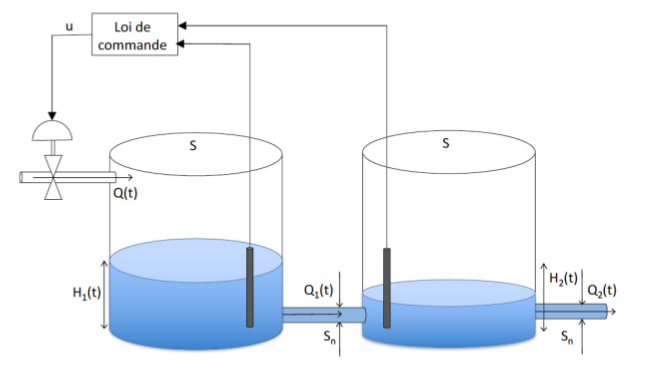
\includegraphics[scale=0.5]{3bac.png}
	\captionof{figure}{\textit{Deux bacs d'eau avec source et fuite\\}}
	\label{fig3} 
	\end{center} 

\section{\textsc{Modélisation du système par un bilan de volume}}

	Nous avons:
\begin{center}

   $ V_1(t)=S\times (H_1(t)-H_2(t))$\\[0.5cm]   
    
  $\dot{V}_1(t)= S \times (\dot{H}_1(t)-\dot{H}_2(t))=(Q(t)-Q_1(t)); \hspace{2mm} Q(t) = S_n \frac{\sqrt{2gH_2}} {K_{debit}}$.\\[0.5cm]
  
    $Q_1(t)=S_n \times v_{n_1} \hspace{3mm}$ avec:$\hspace{1mm}  v^2_{n_1} = 2 \times g\times |H_1(t)-H_2(t)| \\[1 cm]$
 
 Et:
    $V_2(t)=S\times H_2(t)$\\[0.5cm]

   $ \dot{V}_2(t) = S \times \dot{H}_2(t)=(Q_1(t)-Q_2(t)); \hspace{2mm} Q_1(t):$ à trouver\\[0.5cm]
    
    $Q_2(t) = S_n \times v_{n_2} \ ; \hspace{3mm}$ avec:$\hspace{1mm}  v^2_{n_2} = 2 \times g\times H_2(t)$ \\[1 cm]
\end{center} 


Donc $Q_1(t)=S_n\sqrt{2g |H_1(t)-H_2(t)|}$ et $ Q_2(t)=S_n\sqrt{2gH_2(t)} $\\
\par On pose:  $ x_1 = (H_1(t) - H_2(t)) > 0 \hspace{2mm} \forall t$ et $ x_2 = H_2(t) $.\\[0.25 cm]

%\[\Longrightarrow Q_1=S_n\times \sqrt{2\times g \times x_1}\]
%\[\Longrightarrow Q=S_n\times \frac{\sqrt{2\times g \times x_2}}{K_{debit}} \]
%\[\Longrightarrow \dot{x}_1=\frac{Q}{S}-\frac{Q_1}{S}= \frac{S_n\times \sqrt{2\times g }}{S \times K_{debit} } \times \sqrt{x_2} - \frac{S_n\times \sqrt{2\times g }}{S} \times \sqrt{x_1} \] \\[0.5 cm]
%
%\[\Longrightarrow Q_2=S_n\times \sqrt{2\times g \times x_2}\]
%\[\Longrightarrow \dot{x}_2=\frac{Q_1}{S}-\frac{Q_2}{S}= \frac{S_n\times \sqrt{2\times g }}{S} \times \sqrt{x_1} - \frac{S_n\times \sqrt{2\times g }}{S} \times \sqrt{x_2} \]
 
 
 \[\Longrightarrow Q_1=S_n\times \sqrt{2\times g \times x_1}\]
\[\Longrightarrow u=Q=S_n\times \frac{\sqrt{2\times g \times x_2}}{K_{debit}} \]
\[\Longrightarrow \dot{x}_1=\frac{u}{S}-\frac{Q_1}{S}=  \frac{u}{S} - \frac{S_n\times \sqrt{2\times g }}{S} \times \sqrt{x_1} \] \\[0.5 cm]

%\[\Longrightarrow Q_2=S_n\times \sqrt{2\times g \times x_2} = u K_{debit} \]
%\[\Longrightarrow \dot{x}_2=\frac{Q_1}{S}-\frac{K_{debit}}{S} u = \frac{S_n\times \sqrt{2\times g }}{S} \times \sqrt{x_1} - \frac{K_{debit}}{S} u \]
 
\[\Longrightarrow Q_2=S_n\times \sqrt{2\times g \times x_2}\]
\[\Longrightarrow \dot{x}_2=\frac{Q_1}{S}-\frac{Q_2}{S}= \frac{S_n\times \sqrt{2\times g }}{S} \times \sqrt{x_1} - \frac{S_n\times \sqrt{2\times g }}{S} \times \sqrt{x_2} \]

\section{\textsc{Détermination des points d'équilibres}}

 
	  \left \{
   \begin{array}{r c l}
      \dot{x_1}   =  0 \Rightarrow \frac{u}{S}- \frac{Q_1}{S}=  \frac{u}{S} - \frac{S_n\times \sqrt{2\times g }}{S} \times \sqrt{x_1} & =  0\\
      \dot{x_2}   =  0 \Rightarrow \frac{Q_1}{S}-\frac{Q_2}{S} = \frac{S_n\times \sqrt{2\times g }}{S} \times \sqrt{x_1} - \frac{S_n\times \sqrt{2\times g}}{S} \times \sqrt{x_2}  & =  0
   \end{array}
   \right. \\[1 cm]


   \Rightarrow   $x_1_{eq} =  x_2_{eq} $. Il existe un infinité de points d'équilibre.\\
   Rappel: $ x_1 = H_1 - H_2 $ et $ x_2 = H_2 $ \Rightarrow $ H_1 = 2 H_2 $.\\
   
   \section{\textsc{Linéarisation autour de $H^*$}}
   
   \par Puisque $H_1 = 2H_2 = 0.2 $, alors $x_1_{eq} = x_2_{eq} = 0.1 = X_0$.\\    
   
%   \[\dot{\delta_x_1}=f(X_0+\delta_x_1) \indent \Longrightarrow \indent \dot{\delta_x_1}=f(X_0)+\frac{\partial f}{\partial x_1}(X_0).\delta(x_1)\]
%
%	   \[\dot{\delta_x_2}=f(X_0+\delta_x_2) \indent \Longrightarrow \indent \dot{\delta_x_2}=f(X_0)+\frac{\partial f}{\partial x_2}(X_0).\delta(x_2)\] 

$\begin{bmatrix} \dot{\delta_x_1} \\ \dot{\delta_x_2} \end{bmatrix} = \begin{bmatrix} \frac{\partial f_1}{\partial \delta_x_1}_{|X_0}  &  0  \\\\ \frac{\partial f_2}{\partial \delta_x_1}_{|X_0} &  \frac{\partial f_2}{\partial \delta_x_2}_{|X_0}  \end{bmatrix} \begin{bmatrix} \delta_x_1 \\ \delta_x_2 \end{bmatrix} + \begin{bmatrix} \frac{\partial f_1}{\delta_u_1} \\\\ 0  \end{bmatrix} \delta_u $\\[0.5 cm]

$\begin{bmatrix} \dot{\delta_x_1} \\ \dot{\delta_x_2} \end{bmatrix} = \begin{bmatrix} \frac{-S_n}{S} \sqrt{2g} \frac{1}{2\sqrt{0.1}}  &  0 \\\\ \frac{S_n}{S} \sqrt{2g} \frac{1}{2\sqrt{0.1}}  &  \frac{-S_n}{S} \sqrt{2g} \frac{1}{2\sqrt{0.1}}   \end{bmatrix} \begin{bmatrix} \delta_x_1 \\ \delta_x_2 \end{bmatrix} + \begin{bmatrix} \frac{\partial f_1}{\delta_u_1} \\\\ 0  \end{bmatrix} \delta_u$ 
   
 \section{\textsc{Analyse de stabilité asymptotique }}
 
 \par Etudions les valeurs propres du polynôme caractéristique $\Psi(PI_d-A)$:\\ 
   
   \begin{center}
		$ \Psi(PI_d-A) = (p+\frac{S_n}{S} \sqrt{2g} \frac{1}{2\sqrt{0.1}})(p+\frac{S_n}{S} \sqrt{2g} \frac{1}{2\sqrt{0.1}}) =0 $
   \end{center}
   
  
   \par Les valeurs propres obtenues sont:   \left \{
   \begin{array}{r c l}
      p_1  =  p_2  = & -0.022739
   \end{array}
   \right .\\
\par La partie réelle des valeurs propres sont négatives alors le modèle linéaire est asymptotiquement stable.\\ 


\section{\textsc{Fonction de Lyapunov pour le modèle linéaire}}

\par La fonction quadratique: $V(\delta_x)=\frac{\delta_x^2_1}{2}+\frac{\delta_x^2_2}{2}$ qui est définie positive pour $\forall \delta_x \in R $ et qui est de classe $C1$, correspondra à notre fonction de Lyapunov choisie pour notre cas.\\

\par	 Pour rappel:$ X_0 = x_1_{eq} = x_2_{eq} = 0.1$, la dérivée de cette fonction est de cette forme: 
	\begin{center}
		
		%$\dot{V}(\delta_x) = \frac{dV(\delta_x)}{dt} = \frac{dV(\delta_x)}{d\delta_x} \frac{d\delta_x}{dt} = \frac{dV(\delta_x)}{d\delta_x} \dot{\delta_x} $\\[0.25 cm]

		$ \dot{V}(\delta_x) = \delta_x_1 \dot{\delta_x_1}+\delta_x_2 \dot{\delta_x_2}$\\[0.25 cm]

		$ \dot{V}(\delta_x) = \frac{-S_n}{S} \sqrt{\frac{g}{2X_0}}[ \delta_x^2_2 ] $\\[0.25 cm]
		

	\par Cette dérivée,$\dot{V}(\delta_x)$ est définie négative $\dot{V}(\delta_x)<0 \hspace{1mm} \forall \delta_x \in R $. Alors on pourra conclure que le système linéaire est localement asymptotiquement stable.


%\section{\textsc{Fonction de Lyapunov pour le modèle non-linéaire}}
%
%	\par On choisira la même fonction utilisée précédemment soit :$ V(x) \frac{x^2_1}{2}+\frac{x^2_2}{2} $, sa dérivée devient:
%	 
%	\begin{center}
%	
%		
%					
%	\end{center}
%	
%
%	\par De cette façon la fonction dérivée de Lyapunov est définie négative, donc le système est globalement asymptotiquement stable. 
